\documentclass{ximera}
%\handouttrue
\input{../../preamble.tex}

\addPrintStyle{../..}
\begin{document}
    \author{Zomercursus KU Leuven}
    \xmtitle{Oefeningen  Complexe getallen}{}

\providecommand{\shortanswerscols}{3}  % to be removed  when \shortanswercols in preambe.tex ...!

\xmsection{Niveau 1} 

\begin{exercise} 
	\begin{statement}
		Bereken volgende uitdrukkingen. Schrijf de complexe getallen in de vorm $a+bi$.
	\end{statement}	
	\begin{question} $(4+i) + (1-2i) = \answer[onlineshowanswerbutton]{5-i}$
		\begin{oplossing}
			Je kan ofwel reëel en imaginair deel van beide complexe getallen bij elkaar optellen om het antwoord te vinden, ofwel in het complexe vlak de vectorsom maken.
			\begin{image}[0.5\textwidth]
				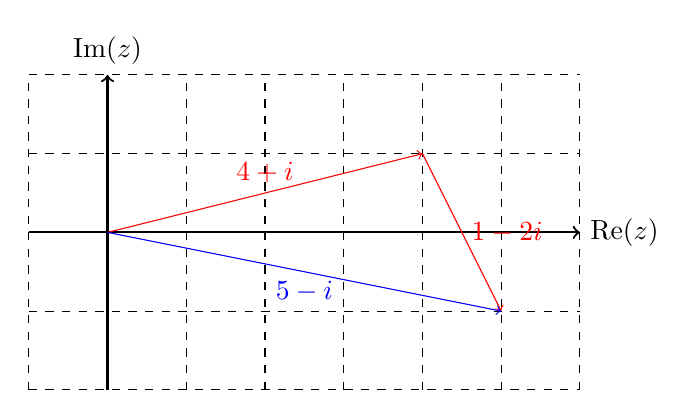
\begin{tikzpicture}[scale=1]
				% grid setup
				
				\def\xmin{-1}
				\def\xmax{6}
				
				\def\ymin{-2}
				\def\ymax{2}				
				
				% grid
				\draw[step = 1.0, black, thin, dashed] (\xmin, \ymin) grid (\xmax, \ymax);
				\draw[->, thick] (\xmin, 0) -- (\xmax, 0) node[right]{Re$(z)$};
				\draw[->, thick] (0, \ymin) -- (0, \ymax) node[above]{Im$(z)$};;	
				
				% tekening
				\draw[->, red]  (0, 0) -- node[above]{$4+i$}  (4,  1);
				\draw[->, red]  (4, 1) -- node[right]{$1-2i$} (5, -1);
				\draw[->, blue] (0, 0) -- node[below]{$5-i$}  (5, -1);	
				\end{tikzpicture}
			\end{image}
		\end{oplossing}
	\end{question}
	

	\begin{question} $(2+3i)(-5+i) = \answer[onlineshowanswerbutton]{-13-13i}$
		\begin{oplossing}
			$$
			(2+3i)(-5+i) = -5 + 2i + 3i\cdot(-5) 3i\cdot i = -13 - 13i
			$$
			\begin{image}[0.5\textwidth]
				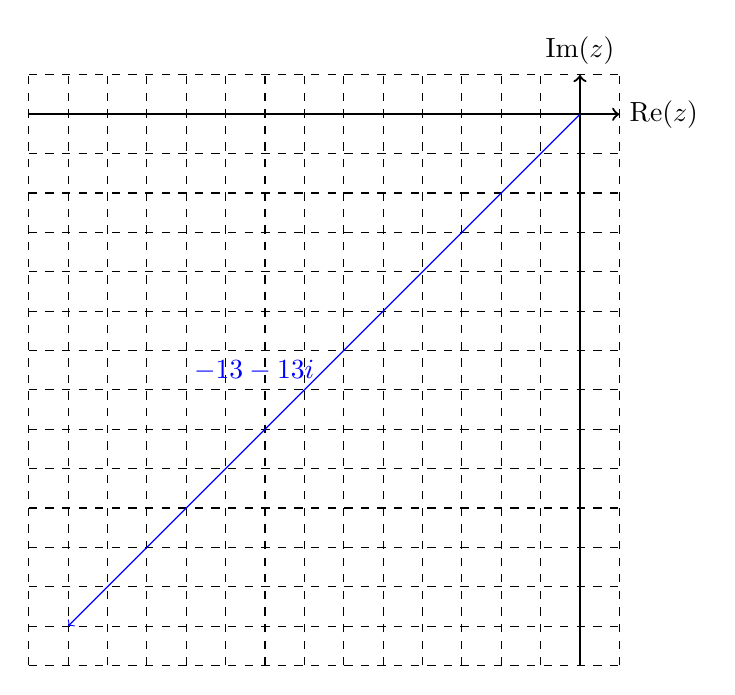
\begin{tikzpicture}[scale=0.5]
				% grid setup
				
				\def\xmin{-14}
				\def\xmax{1}
				
				\def\ymin{-14}
				\def\ymax{1}				
				
				% grid
				\draw[step = 1.0, black, thin, dashed] (\xmin, \ymin) grid (\xmax, \ymax);
				\draw[->, thick] (\xmin, 0) -- (\xmax, 0) node[right]{Re$(z)$};
				\draw[->, thick] (0, \ymin) -- (0, \ymax) node[above]{Im$(z)$};;	
				
				% tekening
				\draw[->, blue] (0, 0) -- node[left]{$-13-13i$}    (-13, -13);	
				\end{tikzpicture}
			\end{image}
		\end{oplossing}
	\end{question}
	
	
	
	\begin{question} $\overline{(3-2i)} = \answer[onlineshowanswerbutton]{3+2i}$
		
	\end{question}
	
	
	
	\begin{question} $|3-2i| = \answer[onlineshowanswerbutton]{\sqrt{13}}$
		\begin{oplossing}
			$|3-2i| = \sqrt{3^2 + 2^2} = \sqrt{13}$ 
		\end{oplossing}
	\end{question}
	
	
	
\end{exercise}

\xmsection{Niveau 2}
\begin{exercise} 
	\begin{statement}
		Bereken volgende uitdrukkingen. Schrijf de complexe getallen in de vorm $a+bi$.
	\end{statement}	
		
		\begin{question} $ (2+4i) - (6-7i) = \answer[onlineshowanswerbutton]{ -4+11i}$
			\begin{oplossing}
				Je kan ofwel reëel en imaginair deel van beide complexe getallen bij elkaar optellen om het antwoord te vinden, ofwel in het complexe vlak de vectorsom maken.
				\begin{image}[0.5\textwidth]
					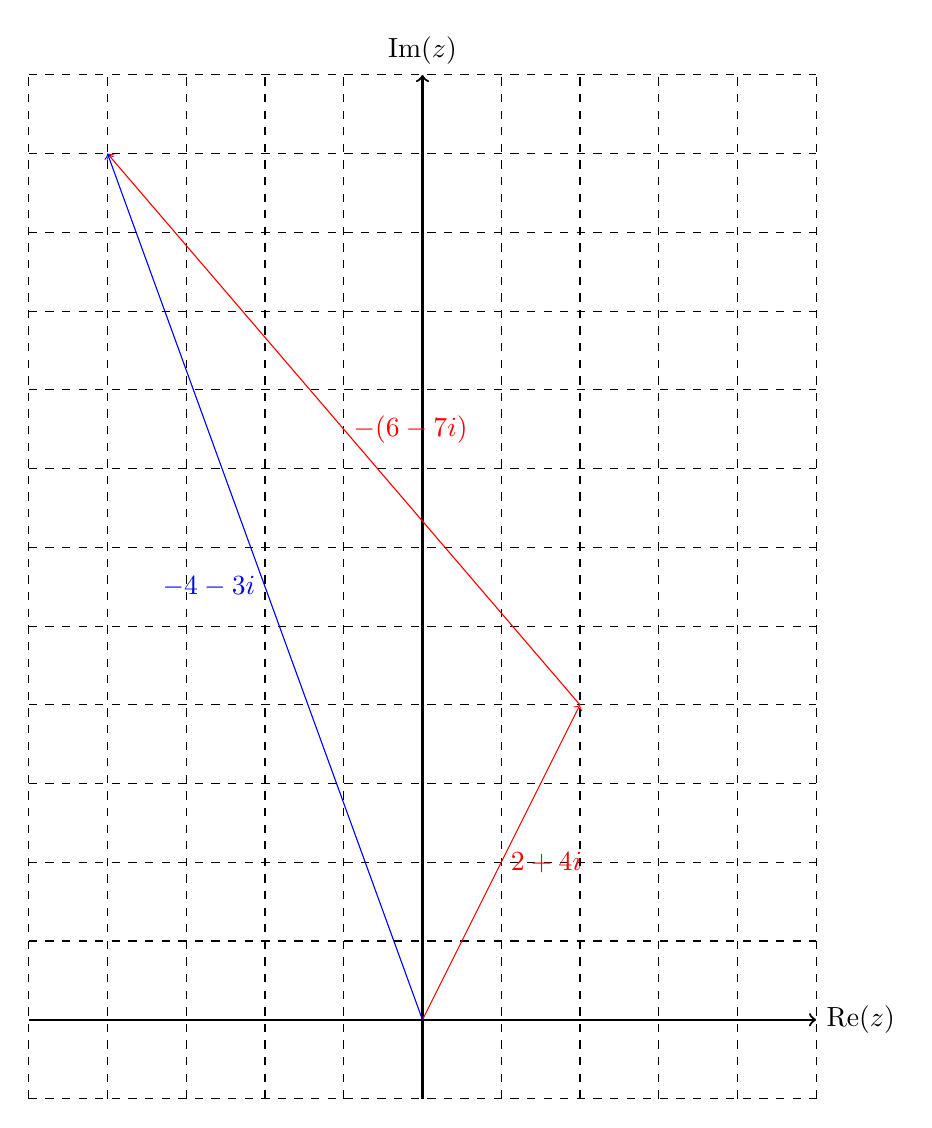
\begin{tikzpicture}[scale=1]
					% grid setup
					
					\def\xmin{-5}
					\def\xmax{5}
					
					\def\ymin{-1}
					\def\ymax{12}				
					
					% grid
					\draw[step = 1.0, black, thin, dashed] (\xmin, \ymin) grid (\xmax, \ymax);
					\draw[->, thick] (\xmin, 0) -- (\xmax, 0) node[right]{Re$(z)$};
					\draw[->, thick] (0, \ymin) -- (0, \ymax) node[above]{Im$(z)$};;	
					
					% tekening
					\draw[->, red]  (0, 0) -- node[right]{$2+4i$}    (2,  4);
					\draw[->, red]  (2, 4) -- node[right]{$-(6-7i)$} (-4, 11);
					\draw[->, blue] (0, 0) -- node[left]{$-4-3i$}   (-4, 11);	
					\end{tikzpicture}
				\end{image}
			\end{oplossing}
		\end{question}
		
		
		
		\begin{question} $(2+i)^2 = \answer[onlineshowanswerbutton]{3+4i}$
			\begin{hint}
				$(a+b)^2 = a^2 + 2ab + b^2$
			\end{hint}
			\begin{oplossing}
				$$
				(2+i)^2  = 4 + 4i + i^2 = 3 + 4i
				$$
				\begin{image}[0.5\textwidth]
					\begin{tikzpicture}[scale=1.3]
					% grid setup
					
					\def\xmin{0}
					\def\xmax{4}
					
					\def\ymin{0}
					\def\ymax{5}				
					
					% grid
					\draw[step = 1.0, black, thin, dashed] (\xmin, \ymin) grid (\xmax, \ymax);
					\draw[->, thick] (\xmin, 0) -- (\xmax, 0) node[right]{Re$(z)$};
					\draw[->, thick] (0, \ymin) -- (0, \ymax) node[above]{Im$(z)$};;	
					
					% tekening
					\draw[->, blue] (0, 0) -- (3, 4) node[above]{$3+4i$};	
					\end{tikzpicture}
				\end{image}
			\end{oplossing}
		\end{question}
		
		\begin{question} $(2+i)+\overline{(3+2i)} = \answer[onlineshowanswerbutton]{5-i}$
			\begin{oplossing}
				Merk op dat $\overline{3+2i} = 3-2i$. Dus moeten we de som $(2+i)+ (3-2i)$ bepalen. Je kan ofwel reëel en imaginair deel van beide complexe getallen bij elkaar optellen om het antwoord te vinden, ofwel in het complexe vlak de vectorsom maken.
				\begin{image}[0.5\textwidth]
					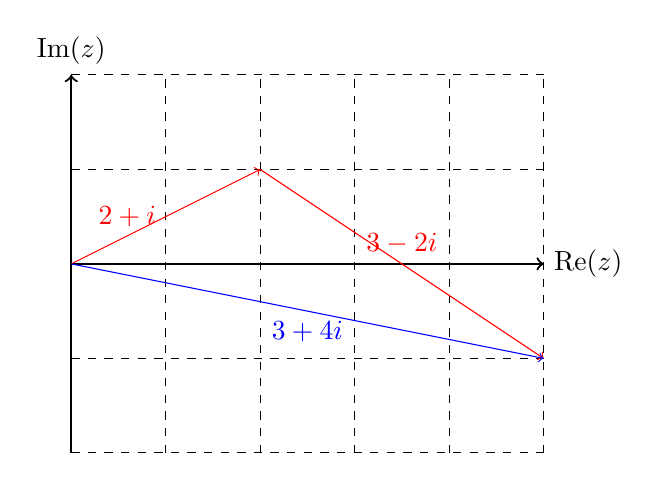
\begin{tikzpicture}[scale=1.2]
					% grid setup
					
					\def\xmin{0}
					\def\xmax{5}
					
					\def\ymin{-2}
					\def\ymax{2}				
					
					% grid
					\draw[step = 1.0, black, thin, dashed] (\xmin, \ymin) grid (\xmax, \ymax);
					\draw[->, thick] (\xmin, 0) -- (\xmax, 0) node[right]{Re$(z)$};
					\draw[->, thick] (0, \ymin) -- (0, \ymax) node[above]{Im$(z)$};;	
					
					% tekening
					\draw[->, red]  (0, 0) -- node[left]{$2+i$}   (2,  1);	
					\draw[->, red]  (2, 1) -- node[above]{$3-2i$} (5, -1);			
					\draw[->, blue] (0, 0) -- node[below]{$3+4i$} (5, -1);	
					\end{tikzpicture}
				\end{image}
			\end{oplossing}
		\end{question}
		
		\begin{question} $(5-6i)(5+6i) = \answer[onlineshowanswerbutton]{61}$
			\begin{oplossing}
				Je kan de rekenregel $z\cdot \overline{z} = |z|^2$ gebruiken. Dan is $(5-6i)(5+6i) = 25 + 36 = 61$.
			\end{oplossing}
		\end{question}
		
				
		\begin{question} $|3-2i + \overline {4-2i}| = \answer[onlineshowanswerbutton]{7}$
			\begin{oplossing}
				Merk eerst op dat $\overline{4-2i} = 4 + 2i$. Je kan ofwel reëel en imaginair deel van beide complexe getallen bij elkaar optellen om de som van twee complexe getallen te vinden, ofwel in het complexe vlak de vectorsom maken.
				\begin{image}[0.5\textwidth]
					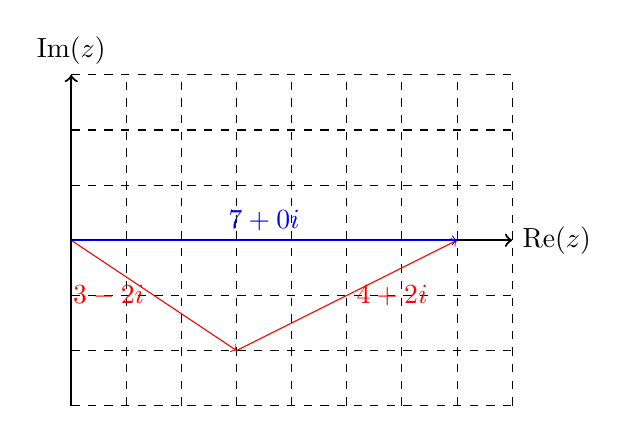
\begin{tikzpicture}[scale=0.7]
					% grid setup
					
					\def\xmin{0}
					\def\xmax{8}
					
					\def\ymin{-3}
					\def\ymax{3}				
					
					% grid
					\draw[step = 1.0, black, thin, dashed] (\xmin, \ymin) grid (\xmax, \ymax);
					\draw[->, thick] (\xmin, 0) -- (\xmax, 0) node[right]{Re$(z)$};
					\draw[->, thick] (0, \ymin) -- (0, \ymax) node[above]{Im$(z)$};;	
					
					% tekening
					\draw[->, red]  (0, 0)  -- node[left]{$3-2i$}  (3,  -2);	
					\draw[->, red]  (3, -2) -- node[right]{$4+2i$}  (7, 0);			
					\draw[->, blue] (0, 0)  -- node[above]{$7+0i$}  (7, 0);	
					\end{tikzpicture}
				\end{image}
				% Aangezien het resultaat een reëel getal is, is de norm van dit getal hetzelfde als de absolute waarde van dit getal, en $|7|= 7$.
			\end{oplossing}
		\end{question}
		
		\begin{question} $|3+4i+4+3i|     = \answer[onlineshowanswerbutton]{7\sqrt 2}$
			\begin{oplossing}
				$|3+4i+4+3i| = |7 + 7i| = \sqrt{49 + 49} = 7 \sqrt{2}$.
			\end{oplossing}
		\end{question}
		
		\begin{question} $|3+4i|+|4+3i| = \answer[onlineshowanswerbutton]{10}$
			\begin{oplossing}
				$|3 + 4i| = \sqrt{3^2 + 4^2} = 5$\\
				$|4+3i| = \sqrt{4^2 + 3^2} = 5$
			\end{oplossing}
		\end{question}
		
		\begin{question} $\left| \frac{(3+4i)(-1+2i)}{(-1-i)(3-i)} \right| =  \answer[onlineshowanswerbutton]{\frac52}$
		\end{question}
		
	\end{exercise}
	
\renewcommand{\shortanswerscols}{1}	
	\begin{exercise}
		%\id{201206wis08*}
		\begin{statement}
		Een complex getal $z$ kunnen we schrijven als $z=a+bi$ met $a$ en $b$ reële getallen en $i^2=-1$.Hoeveel complexe getallen in deze lijst
		\[ 
		\frac{(1+i)^4}{4}, \quad \frac{(1-i)^4}{4}, \quad\frac{(1+i)^2}{2},\quad \frac{(1-i)^2}{2}, \quad i^2 
		\] 
	zijn gelijk zijn aan -1? 
	\end{statement}
 \quad $\answer{3}$
		
		\begin{oplossing}
			Er is al minstens één van deze complexe getallen gelijk aan -1: de laatste, $i^2$, per definitie van de imaginaire eenheid. 
			
			Je kan best te werk gaan door de derde en vierde uitdrukking te bepalen: de eerste twee complexe getallen zijn hun kwadraten. Hiervoor maken we de volgende berekeningen:
			\begin{align*}
			(1+i)^2 &= 1 + 2i + i^2 = 2i  \\
			(1-i)^2 &= 1 - 2i + i^2 = -2i  \\	
			\end{align*}
			en dus vinden we dat
			\begin{align*}
			\frac{(1+i)^2}{2} &= i  \\
			\frac{(1-i)^2}{2} &= -i  \\	
			\end{align*}
			Het derde en vierde complexe getal zijn dus niet gelijk aan -1. Hun kwadraten zijn echter wel gelijk aan -1: drie van de complexe getallen zijn dus gelijk aan -1. 
		\end{oplossing}	
	\end{exercise}

\renewcommand{\shortanswerscols}{3}	
	\begin{exercise}
		\begin{statement}
		Schets in het complexe vlak de gebieden omschreven door volgende vergelijkingen:
		\end{statement}
		\begin{question} 
			$|z| < 1$
			\begin{oplossing} $|z|$ is de afstand van $z$ tot de oorsprong. Alle complexe getallen waarvan de afstand tot de oorsprong kleiner is dan 1 liggen \textit{binnen} een cirkel met straal 1, de rand zelf wordt dus niet meegerekend:
				
				\begin{image}[0.4\textwidth]
					\begin{tikzpicture}[scale=1.4, baseline=(current bounding box.north)]
					
					\draw[->] (-1.2,0) -- (1.2,0) node[right] {Re$(z)$};
					\draw[->] (0,-1.2) -- (0,1.2) node[above] {Im$(z)$};
					
					\draw[white, pattern=north west lines, pattern color=blue] (0,0) circle (1cm);
					\end{tikzpicture}
				\end{image}           
			\end{oplossing}
		\end{question}
		
%		\begin{question} 
%			$|z| \leq 1$
%			\begin{oplossing} $|z|$ is de afstand van $z$ tot de oorsprong. Alle complexe getallen waarvan de afstand tot de oorsprong kleiner is dan of gelijk is aan 1 liggen \textit{binnen} een cirkel met straal 1 waarbij de rand zelf wordt meegerekend:
%				
%				\begin{image}[0.4\textwidth]
%					\begin{tikzpicture}[scale=1.4, baseline=(current bounding box.north)]
%					
%					\draw[->] (-1.2,0) -- (1.2,0) node[right] {Re$(z)$};
%					\draw[->] (0,-1.2) -- (0,1.2) node[above] {Im$(z)$};
%					
%					\draw[blue, thick, pattern=north west lines, pattern color=blue] (0,0) circle (1cm);
%					\end{tikzpicture}
%				\end{image}           
%			\end{oplossing}
%		\end{question}
		
		\begin{question} 
			$|z| = 1$
			\begin{oplossing} $|z|$ is de afstand van $z$ tot de oorsprong. Alle complexe getallen waarvan de afstand tot de oorsprong gelijk is aan 1 liggen dus op een cirkel met straal 1:
				
				\begin{image}[0.4\textwidth]
					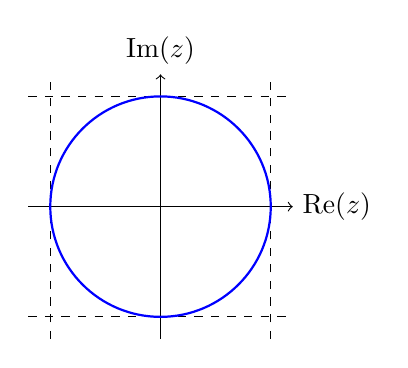
\begin{tikzpicture}[scale=1.4, baseline=(current bounding box.north)]
					
					\draw[dashed, thin] (-1.2,-1.2) grid (1.2, 1.2);
					\draw[->] (-1.2,0) -- (1.2,0) node[right] {Re$(z)$};
					\draw[->] (0,-1.2) -- (0,1.2) node[above] {Im$(z)$};
					
					\draw[blue, thick] (0,0) circle (1cm);
					\end{tikzpicture}
				\end{image}           
			\end{oplossing}
		\end{question}
		
%		\begin{question} 
%			$|z-i| < 1$
%			\begin{oplossing} 
%				Alle complexe getallen waarvoor $|z-i| < 1$ zijn alle complexe getallen $z$ waarvoor de afstand tot $i$ kleiner is dan 1:
%				
%				\begin{image}[0.4\textwidth]
%					\begin{tikzpicture}[scale=1.4, baseline=(current bounding box.north)]
%					
%					\draw[dashed, thin] (-1.2,-1.2) grid (1.2, 2.2);
%					\draw[->] (-1.2, 0) -- (1.2, 0) node[right] {Re$(z)$};
%					\draw[->] (0, -1.2) -- (0, 2.2) node[above] {Im$(z)$};
%					
%					\draw[white, pattern=north west lines, pattern color=blue] (0,1) circle (1cm);	
%					\draw (0,1) node[name=Zi,circle, fill=black, radius=1pt,scale=0.5] {} node [fill=white,xshift=-2pt,left] {$i$};   	
%					\end{tikzpicture}
%				\end{image}  
%			\end{oplossing}
%		\end{question}
		
		\begin{question} 
			$|z-i| \geq 1$
			\begin{oplossing} Alle complexe getallen waarvoor $|z-i| \geq 1$ zijn alle complexe getallen $z$ waarvoor de afstand tot $i$ groter of gelijk is aan 1: 
				\begin{image}[0.4\textwidth]
					\begin{tikzpicture}[scale=1.2, baseline=(current bounding box.north)]
					
					\draw[->] (-2.2, 0) -- (2.2, 0) node[right] {Re$(z)$};
					\draw[->] (0, -1.2) -- (0, 2.2) node[above] {Im$(z)$};
					\draw[pattern=north west lines, pattern color=blue] (-2.2, -1.2) rectangle (2.2, 2.2);
					
					\fill[white] (0,1) circle (1cm);
					\draw[blue, thick] (0,1) circle (1cm);		    
					\draw (0,1) node[name=Zi,circle, fill=black, radius=1pt,scale=0.5] {} node [fill=white,xshift=-2pt,left] {$i$};
					\end{tikzpicture}
				\end{image}            
			\end{oplossing}
		\end{question}
		
		
		
		
		\begin{question} 
			$-1 \leq \text{Im}(z) \leq 2$
			\begin{oplossing} Deze ongelijkheden bepalen een \textit{horizontale} strook, aangezien het imaginaire deel van het complex getal in een interval moet liggen. De randen van de strook behoren tot het geschetste domein.
				
				\begin{image}[0.5\textwidth]
					\begin{tikzpicture}[scale=0.8, baseline=(current bounding box.north)]
					\draw[dashed] (-5, -2) grid (5, 3);
					
					\draw[->, thick] (-5, 0) -- (5, 0) node[right] {Re$(z)$};
					\draw[->, thick] (0, -2) -- (0, 3) node[above] {Im$(z)$};
					
					\draw[white, pattern=north west lines, pattern color=blue] (-5,2) rectangle (5, -1);
					
					% randen toevoegen voor duidelijkheid 
					\draw[blue, thick] (-5, -1) -- (5, -1);
					\draw[blue, thick] (-5, 2) -- (5, 2);
					\end{tikzpicture}
				\end{image}
			\end{oplossing}            
		\end{question}  
		
		
		
		
		\begin{question} 
			$\text{Re}(z)> \text{Im}(z)>0$
			\begin{oplossing} 
				Als $z=a+bi$, dan betekent $\text{Re}(z) > \text{Im}(z) > 0$ dat $a > b > 0$. Dit is het gebied onder de rechte $y = x$, (daar is $a > b$), en boven de $x$-as (daar is $b > 0$):
				
				\begin{image}[0.4\textwidth]
					\begin{tikzpicture}[scale=1.1, baseline=(current bounding box.north)]
					\draw[dashed] (-0.5, -0.5) grid (2.9, 2.9);
					
					\draw[->, thick] (-0.5, 0) -- (2.9, 0) node[right] {Re$(z)$};
					\draw[->, thick] (0, -0.5) -- (0, 2.9) node[above] {Im$(z)$};
					
					\draw[white, pattern=north west lines, pattern color=blue] (0,0.02) -- (2.9, 2.9) -- (2.9, 0.02) -- cycle;
					\end{tikzpicture}
				\end{image}       
			\end{oplossing}
		\end{question}
		
		
	\end{exercise}

\renewcommand{\shortanswerscols}{2}	
	\begin{exercise}
		\begin{statement}
		Voer volgende delingen uit door de opgave te schrijven in de vorm $a+bi$.
		\end{statement}
		\begin{question}$ \frac{7}{i} = \answer[onlineshowanswerbutton]{-7i}$
			\begin{oplossing}
				We vermenigvuldigen teller en noemer met $\overline{i} = -i$. In de noemer krijgen we dan $i\cdot (-i) = 1$. Het resultaat is $-7i$. Voor oefeningen kan het handig zijn om te onthouden dat \textit{delen door $i$ hetzelfde is als vermenigvuldigen met $-i$}. % IDEE: dit laatste misschien ook eens bespreken en duidelijk maken in theorie blokje? 
			\end{oplossing}
		\end{question}
		
		\begin{question}$ \frac{1}{5+2i} = \answer[onlineshowanswerbutton]{\frac{5}{29}-\frac{2}{29}i}$
			\begin{oplossing}
				We vermenigvuldigen teller en noemer met $\overline{5+2i} = 5-2i$. In de noemer krijgen we dan $(5+2i)(5-2i) = 29$.
				$$
				\frac{1}{5+2i} = \frac{1}{5+2i} \frac{5-2i}{5-2i} = \frac{5-2i}{25}=\frac{5}{29}-\frac{2}{29}i
				$$
			\end{oplossing}
		\end{question}
		
		\begin{question} $ \frac{1+i}{2+3i}	= \answer[onlineshowanswerbutton]{\frac{5}{13}-\frac{1}{13}i}$
			\begin{oplossing}
				We vermenigvuldigen teller en noemer met $\overline{2+3i} = 2-3i$. In de noemer krijgen we dan $(2+3i)(2-3i) = 13$.
				$$
				\frac{1+i}{2+3i} = \frac{1+i}{2+3i} \cdot \frac{2-3i}{2-3i} = \frac{5-i}{13}=\frac{5}{13}-\frac{1}{13}i
				$$
			\end{oplossing}
		\end{question}
		
		
		\begin{question} $ \frac{1+2i}{3-4i} + \frac{2-i}{5i} = \answer[onlineshowanswerbutton]{-\frac{2}{5}}$
			\begin{oplossing}
				We berekenen de beide termen apart, en tellen de resultaten vervolgens bij elkaar op.
				
				Voor de eerste term: we vermenigvuldigen teller en noemer met $\overline{3-4i} = 3+4i$. In de noemer krijgen we dan $(3-4i)(3+4i) = 25$. De eerste term kunnen we dus vereenvoudigen tot
				$$
				\frac{1+2i}{3-4i} = \frac{1+2i}{3-4i} \cdot \frac{3+4i}{3+4i} = \frac{-5+10i}{25} = \frac{-1+2i}{5}
				$$
				
				Voor de tweede term: we vermenigvuldigen teller en noemer met $\overline{5i} = -5i$. In de noemer krijgen we dan $(5i)\cdot(-5i) = 25$. De tweede term kunnen we dus vereenvoudigen tot
				$$
				\frac{2-i}{5i} = \frac{2-i}{5i} \cdot \frac{-5i}{-5i} = \frac{-1-2i}{5}
				$$
				Een andere mogelijkheid is om te gebruiken dat delen door $i$ hetzelfde is als vermenigvuldigen met $-i$, zodat we meteen bekomen dat
				$$
				\frac{2-i}{5i} = \frac{(2-i)\cdot (-i)}{5} = \frac{-1-2i}{5}
				$$
				
				Wanneer we deze twee termen bij elkaar optellen, valt het imaginaire deel weg. Het resultaat is $\frac{-2}{5}$. 
			\end{oplossing}
		\end{question}
	\end{exercise}
	
	
	\begin{exercise}
		\begin{statement}
		Bepaal alle oplossingen van volgende veeltermvergelijkingen.
		\end{statement}
		
		
		\begin{question}
			$ x^2 + x = 0$
			\begin{uitkomst} $x_1 = 0$ en $x_2 = -1$
				\end{uitkomst}
			\begin{oplossing}
				De oplossingen zijn $x_1 = 0$ en $x_2 = -1$.
				
				We kunnen een $x$ afzonderen in deze vergelijking en vinden dan de equivalente vergelijking $x(x+1) = 0$. Deze heeft als oplossingen $x=0$ en $x=-1$.
			\end{oplossing}
		\end{question}
		
		\begin{question}
			$ x^3 + 16x = 0$
			\begin{uitkomst} $x_1 = 0$, $x_2 = 4i$ en $x_3 = -4i$
				\end{uitkomst}
			\begin{oplossing}
				De oplossingen zijn $x_1 = 0$, $x_2 = 4i$ en $x_3 = -4i$.
				
				We kunnen een $x$ afzonderen, en vinden dan de equivalente vergelijking $x(x^2+16)=0$. Deze heeft als oplossingen ofwel $x=0$ ofwel $x^2 + 16 = 0$. De laatste vergelijking heeft als oplossingen $x=4i$ en $x=-4i$.
			\end{oplossing}
		\end{question}
		
		
		\begin{question}
			$ x^2 + 5x + 2 = 0$
			\begin{uitkomst} $x_1 = \frac{-5 + \sqrt{17}}{2}$ en $x_2 = \frac{-5 - \sqrt{17}}{2}$
			\end{uitkomst}
			\begin{oplossing}
				De oplossingen zijn $x_1 = \frac{-5 + \sqrt{17}}{2}$ en $x_2 = \frac{-5 - \sqrt{17}}{2}$.
				
				De vergelijking is van de vorm $ax^2 + bx + c = 0$, met $a=1$, $b=5$ en $c=2$. Dan is $D = b^2 - 4ac = 25-8 = 17$. Omdat $D > 0$, zijn er twee reële oplossingen:
				$$
				x_1 = \frac{-b + \sqrt{D}}{2a} = \frac{-5 + \sqrt{17}}{2}, \ \ x_2 = \frac{-b - \sqrt{D}}{2a} = \frac{-5 - \sqrt{17}}{2} \, .
				$$
			\end{oplossing}
		\end{question}
		
		\begin{question}
			$ x^2 + 4x + 5 = 0$
			\begin{uitkomst} $x_1 = -2 - i$ en $x_2 = -2 + i$
			\end{uitkomst}
			\begin{oplossing}
				De oplossingen zijn $x_1 = -2 - i$ en $x_2 = -2 + i$.
				
				De vergelijking is van de vorm $ax^2 + bx + c = 0$, met $a=1$, $b=4$ en $c=5$. Dan is $D = b^2 - 4ac = 16 - 20 = -4$. Omdat $D < 0$, zijn er twee complexe oplossingen. De oplossingen zijn
				$$
				x_1 = \frac{-b + i\sqrt{-D}}{2a} = \frac{-4 + 2i}{2} = -2 + i, \ \ x_2 = \frac{-b - i\sqrt{-D}}{2a} = \frac{-4 - 2i}{2} = -2 - i \, .
				$$
			\end{oplossing}
		\end{question}
		
		
		
		
%		\begin{question}
%			$ 9x^2 - 14 = 4x$
%			\begin{uitkomst} $x_1 = \frac{2 + \sqrt{130}}{9}$ en $x_2 = \frac{2 - \sqrt{130}}{9}$
%			\end{uitkomst}
%			\begin{oplossing}
%				De oplossingen zijn $x_1 = \frac{2 + \sqrt{130}}{9}$ en $x_2 = \frac{2 - \sqrt{130}}{9}$.
%				
%				De vergelijking is van de vorm $ax^2 + bx + c = 0$, met $a=9$, $b=-4$ en $c=-14$. Dan is $D = b^2 - 4ac = 16 + 504 = 520$. Omdat $D > 0$, zijn er twee verschillende reële oplossingen. Merk op dat $\sqrt{D} = \sqrt{520} = \sqrt{4 \cdot 130} = 2 \sqrt{130}$. De oplossingen zijn
%				$$
%				x_1 = \frac{-b + \sqrt{D}}{2a} = \frac{4 + 2 \sqrt{130}}{18} = \frac{2 + \sqrt{130}}{9}, \ \ x_2 = \frac{-b - \sqrt{D}}{2a} = \frac{4 - 2 \sqrt{130}}{18} = \frac{2 - \sqrt{130}}{9}\, .
%				$$
%			\end{oplossing}
%		\end{question}
		
		\begin{question}
			$ x = 2x^2 + 5$
			\begin{uitkomst} $x_1 = \frac{1}{4} + \frac{\sqrt{39}}{4} i$ en $x_2 = \frac{1}{4} - \frac{\sqrt{39}}{4} i$
			\end{uitkomst}
			\begin{oplossing}
				De oplossingen zijn $x_1 = \frac{1}{4} + \frac{\sqrt{39}}{4} i$ en $x_2 = \frac{1}{4} - \frac{\sqrt{39}}{4} i$.
				
				De vergelijking is van de vorm $ax^2 + bx + c = 0$, met $a=2$, $b=-1$ en $c=5$. Dan is $D = b^2 - 4ac = 1 - 40 = -39$. Omdat $D < 0$, zijn er twee complexe oplossingen. De oplossingen zijn
				$$
				x_1 = \frac{-b + i\sqrt{-D}}{2a} = \frac{1 + \sqrt{39}i}{4} = \frac{1}{4} + \frac{\sqrt{39}}{4} i, \ \ x_2 = \frac{-b - i\sqrt{-D}i}{2a} = \frac{1 - \sqrt{39}i}{4} = \frac{1}{4} - \frac{\sqrt{39}}{4} i \, .
				$$
			\end{oplossing}
		\end{question}
		
	\end{exercise}
	

\begin{exercise}
	\begin{statement}
	Schrijf onderstaande getallen in goniometrische vorm $r(\cos\theta+i\sin \theta)$. Zorg er steeds voor dat $\theta$ tussen 0 en $2\pi$ ligt, dus niet $-\frac{\pi}{2}$ antwoorden maar $\frac{3\pi}{2}$.
	\end{statement}
%	\begin{question}  $z=1$ 
%		\begin{uitkomst} $z =  \cos 0 + i\sin 0$
%			\end{uitkomst}
%		\begin{oplossing} 
%			Omdat $z = 1 = 1 + 0i$ en dus $a = 0$ en $b = 1$, vinden we $|z| = r = 1$. In het complexe vlak zien we dadelijk dat $\theta = 0$.
%			%Bovendien voldoet $\theta$ aan $\cos \theta = 1$ en $\sin \theta = 0$ zodat $\theta = 0$. 
%			De goniometrische schrijfwijze van $z$ is dan $z = 1 =  \cos 0 + i\sin 0$.
%			\begin{image}[0.5\textwidth]
%				\begin{tikzpicture}[scale = 1, trig format = rad]
%				%	grid setup
%				
%				\def\xmin{-2}
%				\def\xmax{2}
%				
%				\def\ymin{-2}
%				\def\ymax{2}				
%				
%				%	grid
%				\draw[step = 1, black, thin, dashed] (\xmin, \ymin) grid (\xmax, \ymax);
%				\draw[->] (\xmin, 0) -- (\xmax, 0) node[right]{Re$(z)$};
%				\draw[->] (0, \ymin) -- (0, \ymax) node[above]{Im$(z)$};;	
%				
%				%	vector
%				\draw[->, blue, very thick] (0, 0) -- node[below]{$1$}(1, 0);
%				
%				%	boogje - niet handig nu
%				\def\r{0.2}
%				%\draw[->, blue] (\r, 0) arc (0:0:\r) node[right]{$0$};
%				\end{tikzpicture}
%			\end{image}
%		\end{oplossing}
%	\end{question}
	
	\begin{question} 
		 $z=-1$ 
		\begin{uitkomst} $z  = \cos \pi + i\sin \pi$
		\end{uitkomst}
		\begin{oplossing} 
			$z=-1 = -1 + 0i$ en dus $a = -1$ en $b = 0$, waaruit we halen dat $|z| = r = 1$. In het complexe vlak zien we dadelijk dat $\theta = \pi$. 
			%Het argument van $z$ moet voldoen aan $\cos \theta = -1$ en $\sin \theta = 0$ zodat $\theta = \pi$. 
			De goniometrische schrijfwijze van $z$ is dan $z  = \cos \pi + i\sin \pi$.
			\begin{image}[0.5\textwidth]
				\begin{tikzpicture}[scale = 1]
				%	grid setup
				
				\def\xmin{-2}
				\def\xmax{2}
				
				\def\ymin{-2}
				\def\ymax{2}				
				
				%	grid
				\draw[step = 1, black, thin, dashed] (\xmin, \ymin) grid (\xmax, \ymax);
				\draw[->] (\xmin, 0) -- (\xmax, 0) node[right]{Re$(z)$};
				\draw[->] (0, \ymin) -- (0, \ymax) node[above]{Im$(z)$};;	
				
				%	vector
				\draw[->, blue, very thick] (0, 0) -- node[below]{$-1$}(-1, 0);
				
				%	boogje - niet handig nu
				\def\r{0.2}
				\draw[->, blue] (\r, 0) arc (0:180:\r) node[midway, above]{$\pi$};
				\end{tikzpicture}
			\end{image}
			Merk op dat de modules positief moet zijn, en met $r=-1$ en $\theta = 0$ is $-(\cos 0 + i\sin0)$ dus \textit{geen} goniometrische schrijfwijze van het getal $-1$.
		\end{oplossing}
	\end{question}
	
%	\begin{question} 
%		 $z = i$ 
%		\begin{uitkomst} $z = \cos \frac{\pi}{2} +i\sin \frac{\pi}{2}$
%		\end{uitkomst}
%		\begin{oplossing} 
%			Omdat $z = i = 0 + i$, en dus $a = 0$, $b = 1$, zodat $|z| = r = 1$. In het complexe vlak zien we dadelijk dat $\theta=\frac{\pi}{2}$.
%			% en $\theta$ voldoet aan $\cos\theta = 0$ en $\sin \theta = 1$ (of je kan het ook afleiden uit onderstaande schets). 
%			De goniometrische schrijfwijze van $z$ is dus $z = \cos \frac{\pi}{2} +i\sin \frac{\pi}{2}$.
%			\begin{image}[0.5\textwidth]
%				\begin{tikzpicture}[scale = 1]
%				%	grid setup
%				
%				\def\xmin{-2}
%				\def\xmax{2}
%				
%				\def\ymin{-2}
%				\def\ymax{2}				
%				
%				%	grid
%				\draw[step = 1, black, thin, dashed] (\xmin, \ymin) grid (\xmax, \ymax);
%				\draw[->] (\xmin, 0) -- (\xmax, 0) node[right]{Re$(z)$};
%				\draw[->] (0, \ymin) -- (0, \ymax) node[above]{Im$(z)$};;	
%				
%				%	vector
%				\draw[->, blue, very thick] (0, 0) -- node[left]{$i$}(0, 1);
%				
%				%	boogje
%				\def\r{0.2}
%				\draw[->, blue] (\r, 0) arc (0:90:\r) node[midway, right]{$\pi/2$};
%				\end{tikzpicture}
%			\end{image}
%			
%		\end{oplossing}
%	\end{question}
	
	\begin{question} 
		 $z = -i$ 
		\begin{uitkomst} $z  = \cos\left(\frac{3\pi}{2}\right) +i \sin\left(\frac{3\pi}{2}\right)$
		\end{uitkomst}
		\begin{oplossing}
			Voor $z = -i$ is $a = 0$ en $b = -1$, dus $|z| = r = 1$. In het complexe vlak zien we dadelijk dat $\theta=\frac{3\pi}{2}$.
			% en $\theta$ voldoet aan $\cos \theta = 0$ en $\sin \theta = -1$, dus $\theta = - \frac{\pi}{2} = \frac{3\pi}{2}$. 
			De goniometrische schrijfwijze van $z$ is dus $z  = \cos\left(\frac{3\pi}{2}\right) +i \sin\left(\frac{3\pi}{2}\right)$.
			\begin{image}[0.5\textwidth]
				\begin{tikzpicture}[scale = 1]
				%	grid setup
				
				\def\xmin{-2}
				\def\xmax{2}
				
				\def\ymin{-2}
				\def\ymax{2}				
				
				%	grid
				\draw[step = 1, black, thin, dashed] (\xmin, \ymin) grid (\xmax, \ymax);
				\draw[->] (\xmin, 0) -- (\xmax, 0) node[right]{Re$(z)$};
				\draw[->] (0, \ymin) -- (0, \ymax) node[above]{Im$(z)$};;	
				
				%	vector
				\draw[->, blue, very thick] (0, 0) -- node[right]{$-i$}(0, -1);
				
				%	boogje
				\def\r{0.2}
				\draw[->, blue] (\r, 0) arc (0:270:\r) node[midway, above]{$\frac{3\pi}{2}$};
				\end{tikzpicture}
			\end{image}
		\end{oplossing}
	\end{question}
	
	\begin{question} 
		$z = \sqrt{3} + i$ 
		\begin{uitkomst} $
			z = 2\left(\cos \left(\frac{\pi}{6}\right) + i\sin\left(\frac{\pi}{6}\right)\right) \, .
			$
		\end{uitkomst}
		\begin{oplossing} 
			Voor $z = \sqrt{3} + i$ geldt $a = \sqrt{3}$ en $b = 1$, dus $|z| = r = \sqrt{a^2 + b^2} = 2$. Het argument van $z$ voldoet aan $\cos \theta = \frac{\sqrt{3}}{2}$ en $\sin \theta = \frac{1}{2}$. Dit zijn de goniometrische getallen van de standaardhoek $\pi/6$. De goniometrische schrijfwijze van $z$ is dus 
			$$
			z = 2\left(\cos \left(\frac{\pi}{6}\right) + i\sin\left(\frac{\pi}{6}\right)\right) \, .
			$$
			\begin{image}[0.5\textwidth]
				\begin{tikzpicture}[scale = 1.5]
				%	grid setup
				
				\def\xmin{-2.1}
				\def\xmax{2.1}
				
				\def\ymin{-2.1}
				\def\ymax{2.1}				
				
				%	grid
				\draw[step = 1, black, thin, dashed] (\xmin, \ymin) grid (\xmax, \ymax);
				\draw[->] (\xmin, 0) -- (\xmax, 0) node[right]{Re$(z)$};
				\draw[->] (0, \ymin) -- (0, \ymax) node[above]{Im$(z)$};;	
				
				%	vector
				\draw[->, blue, very thick] (0, 0) -- ({sqrt(3)}, 1)node[below]{$\sqrt{3} + i$};
				
				%	boogje
				\def\r{0.5}
				\draw[->, blue] (\r, 0) arc (0:30:\r) node[midway, right]{$\frac{\pi}{6}$};
				\end{tikzpicture}
			\end{image}
		\end{oplossing}
	\end{question}
	
	\begin{question} 
		 $z = -\sqrt{3} + i$ 
		\begin{uitkomst} $
			z = 2\left(\cos \left(\frac{5\pi}{6}\right) + i\sin\left(\frac{5\pi}{6}\right)\right) \, .
			$
		\end{uitkomst}
		\begin{oplossing} 
			Voor $z = -\sqrt{3} + i$ geldt $a = -\sqrt{3}$ en $b = 1$. Dus geldt $|z| = r = 2$. Voor het argument van $z$ geldt dat $\cos \theta = -\frac{\sqrt{3}}{2}$ en $\sin \theta = \frac{1}{2}$. Dan is $\theta =  \frac{5\pi}{6} =\pi -  \frac{\pi}{6}$: dit kan je afleiden uit de goniometrische getallen voor $\pi/6$ en de rekenregels voor supplementaire hoeken te gebruiken.
			
			De goniometrische schrijfwijze van $z$ is dus 
			$$
			z = 2\left(\cos \left(\frac{5\pi}{6}\right) + i\sin\left(\frac{5\pi}{6}\right)\right) \, .
			$$
			
			\begin{image}[0.5\textwidth]
				\begin{tikzpicture}[scale = 1.5]
				%	grid setup
				
				\def\xmin{-2.1}
				\def\xmax{2.1}
				
				\def\ymin{-2.1}
				\def\ymax{2.1}				
				
				%	grid
				\draw[step = 1, black, thin, dashed] (\xmin, \ymin) grid (\xmax, \ymax);
				\draw[->] (\xmin, 0) -- (\xmax, 0) node[right]{Re$(z)$};
				\draw[->] (0, \ymin) -- (0, \ymax) node[above]{Im$(z)$};;	
				
				%	vector
				\draw[->, blue, very thick] (0, 0) -- ({-sqrt(3)}, 1)node[below]{$-\sqrt{3} + i$};
				
				%	boogje
				\def\r{0.5}
				\draw[->, blue] (\r, 0) arc (0:150:\r) node[midway, above]{$5\pi/6$};
				\end{tikzpicture}
			\end{image}
		\end{oplossing}
	\end{question}
	
	
\end{exercise}

\begin{exercise}
	\begin{statement}
	Bepaal de modulus $|z|$ en het argument $\theta$ van volgende complexe getallen $z$. Geef de hoek $\theta$ tussen 0 en $2\pi$ radialen.
	\end{statement}
	\begin{question} 
		 $z=-7i$
		\begin{uitkomst}  $|z|=7$ en $\theta=3\pi/2$.
			\end{uitkomst}
		\begin{oplossing}
			$z = a + bi = 0 - 7i$, dus is $|z| = \sqrt{a^2 + b^2} = 7$. In het complexe vlak zien we dadelijk dat $\theta = 3 \pi/2$.  Je kan dit ook berekenen:  $\cos\theta=0/7=0$ en $\sin\theta=-7/7=-1$, en dus is $\theta = 3 \pi/2$ (op een veelvoud van $2\pi$ na). 
			
			\begin{image}[0.5\textwidth]
				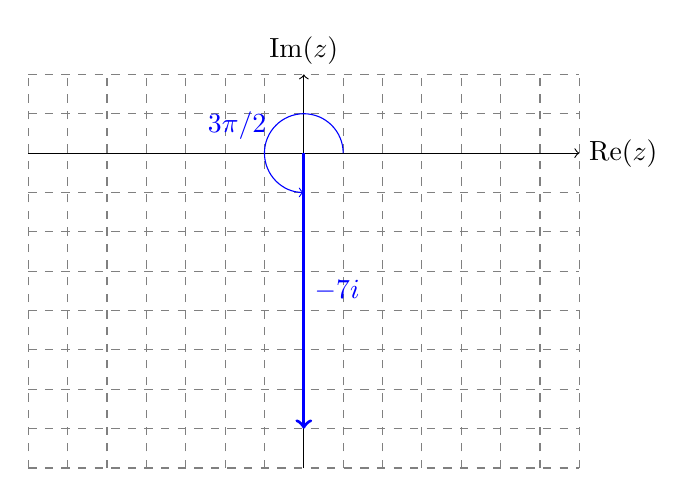
\begin{tikzpicture}[scale = 0.5]
				%	grid setup
				
				\def\xmin{-7}
				\def\xmax{7}
				
				\def\ymin{-8}
				\def\ymax{2}				
				
				%	grid
				\draw[step = 1.0, gray, thin, dashed] (\xmin, \ymin) grid (\xmax, \ymax);
				\draw[->] (\xmin, 0) -- (\xmax, 0) node[right]{Re$(z)$};
				\draw[->] (0, \ymin) -- (0, \ymax) node[above]{Im$(z)$};;	
				
				%	vector
				\draw[->, blue, very thick] (0, 0) -- node[right]{$-7i$}  (0, -7);
				
				%	boogje
				\def\r{1}
				\draw[->, blue] (\r, 0) arc (0:270:\r) node[midway, left]{$3\pi/2$};
				\end{tikzpicture}
			\end{image}
		\end{oplossing}
	\end{question}
	
	
	\begin{question} 
		 $z=(7i)^{-1}$
		\begin{uitkomst}  $|z|=1/7$ en $\theta=3\pi/2$.
		\end{uitkomst}
		\begin{hint} Schrijf $z$ eerst in cartesische vorm $a+bi$. \end{hint}
		\begin{oplossing}
			Eerst herschrijven we het complex getal $z$ in cartesische vorm: $z = \frac{1}{7i} = - \frac17 i$ (vermenigvuldig teller en noemer met $i$). 
			\\
			Een tip voor berekeningen met complexe getallen: \textit{delen door $i$ is hetzelfde als vermenigvuldigen met $-i$}.
			
			Omdat $z = a + bi = 0 - \frac17i$ is $|z| = \sqrt{a^2 + b^2} = \frac17$, en $\theta = 3 \pi/2$ (op een veelvoud van $2\pi$ na), zoals we kunnen afleiden uit een schets (de ijk op beide assen is nu 0.1 in plaats van 1):
			
			\begin{image}[0.5\textwidth]
				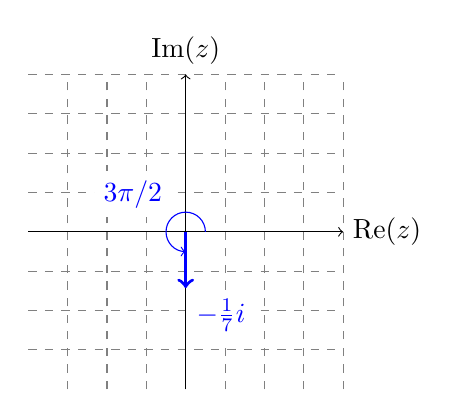
\begin{tikzpicture}[scale = 5]
				%	grid setup
				
				\def\xmin{-0.4}
				\def\xmax{0.4}
				
				\def\ymin{-0.4}
				\def\ymax{0.4}				
				
				%	grid
				\draw[step = 0.1, gray, thin, dashed] (\xmin, \ymin) grid (\xmax, \ymax);
				\draw[->] (\xmin, 0) -- (\xmax, 0) node[right]{Re$(z)$};
				\draw[->] (0, \ymin) -- (0, \ymax) node[above]{Im$(z)$};;	
				
				%	vector
				\draw[->, blue, very thick] (0, 0) -- (0, -1/7) node[below right, fill = white]{$-\frac17i$};
				
				%	boogje
				\def\r{0.05}
				\draw[->, blue] (\r, 0) arc (0:270:\r) node[midway, above left, fill = white]{$3\pi/2$};
				\end{tikzpicture}
			\end{image}
		\end{oplossing}
	\end{question}
	
	
	\begin{question} 
		 $z = \overline{1+i}$
		\begin{uitkomst} $|z| = \sqrt{2}$ en $\theta = 7\pi/4$.
		\end{uitkomst}
		\begin{hint} Schrijf $z$ eerst in cartesische vorm $a+bi$. \end{hint}
		\begin{oplossing}
			Eerst herschrijven we het complex getal $z$: $z = \overline{1+i} = 1 - i$.
			
			Omdat $z = a + bi = 1 - i$, is $|z| = \sqrt{a^2 + b^2} = \sqrt{2}$, en $\theta =- \pi / 4$: dit kan je afleiden uit de tekening of bepaal je uit de vergelijkingen 
			%$a = r\cos \theta$ en $b = r\sin\theta$. Deze kan je omvormen naar
			\begin{align*}
			\cos \theta &= \frac{a}{r} = \frac{1}{\sqrt{2}} \\
			\sin \theta &= \frac{b}{r} = -\frac{1}{\sqrt{2}}\\
			\end{align*} 
			We weten dat de cosinus en sinus van de standaardhoek $\pi/4$ beide gelijk zijn aan $\frac{1}{\sqrt{2}}=\frac{\sqrt2}{2}$, en de tegengestelde hoek heeft dezelfde cosinus, maar een tegengestelde sinus. Dus $\theta = - \pi/4$ of $\theta= 7 \pi/4$.
			\begin{image}[0.5\textwidth]
				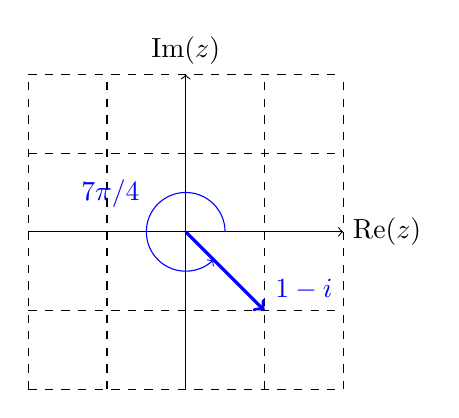
\begin{tikzpicture}[scale = 1]
				%	grid setup
				
				\def\xmin{-2}
				\def\xmax{2}
				
				\def\ymin{-2}
				\def\ymax{2}				
				
				%	grid
				\draw[step = 1, black, thin, dashed] (\xmin, \ymin) grid (\xmax, \ymax);
				\draw[->] (\xmin, 0) -- (\xmax, 0) node[right]{Re$(z)$};
				\draw[->] (0, \ymin) -- (0, \ymax) node[above]{Im$(z)$};;	
				
				%	vector
				\draw[->, blue, very thick] (0, 0) --  (1, -1) node[above right]{$1-i$};
				
				%	boogje
				\def\r{0.5}
				\draw[->, blue] (\r, 0) arc (0:315:\r) node[midway, above left]{$7\pi/4$};
				\end{tikzpicture}
			\end{image}
		\end{oplossing}
	\end{question}
	
	
	\begin{question} 
		 $z = \dfrac{1-i}{1+i}$
		\begin{uitkomst}  $|z| = 1$ en $\theta=3\pi/2$.
		\end{uitkomst}
		\begin{hint} Schrijf $z$ eerst in cartesische vorm $a+bi$. \end{hint}
		\begin{oplossing}
			Eerst herschrijven we het complex getal $z$ naar de vorm $a + bi$:
			$$
			\frac{1-i}{1+i} = \frac{1-i}{1+i} \frac{1-i}{1-i} = \frac{(1-i)^2}{2}= \frac{-2i}{2} = - i 
			$$
			Dan is $|z| = 1$, en in het comlexe vlak zien we dadelijk dat $\theta = 3 \pi/2$.
			\begin{image}[0.5\textwidth]
				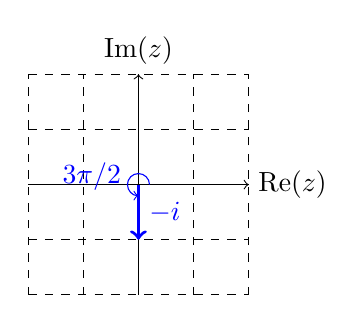
\begin{tikzpicture}[scale = 0.7]
				%	grid setup
				
				\def\xmin{-2}
				\def\xmax{2}
				
				\def\ymin{-2}
				\def\ymax{2}				
				
				%	grid
				\draw[step = 1, black, thin, dashed] (\xmin, \ymin) grid (\xmax, \ymax);
				\draw[->] (\xmin, 0) -- (\xmax, 0) node[right]{Re$(z)$};
				\draw[->] (0, \ymin) -- (0, \ymax) node[above]{Im$(z)$};;	
				
				%	vector
				\draw[->, blue, very thick] (0, 0) -- node[right]{$-i$}  (0, -1);
				
				%	boogje
				\def\r{0.2}
				\draw[->, blue] (\r, 0) arc (0:270:\r) node[midway, left]{$3\pi/2$};
				\end{tikzpicture}
			\end{image}
		\end{oplossing}
	\end{question}    
	
	%%% Volgende oefening in comment: geen standaardhoek, is minder interessant.
	
	
	%\begin{question} 
	%Als $z = \dfrac{1}{1+i}+\dfrac{1+i}{4}$, dan is $|z| = \answer[onlineshowanswerbutton]{\sqrt{10}/4}$ en $\theta=\answer[onlineshowanswerbutton]{-0.32}$.
	%\begin{hint}
	%Om $\theta$ te berekenen, gebruik je best een rekenmachine.
	%\end{hint}
	%\begin{oplossing}
	%Eerst herschrijven we het complex getal $z$ naar de vorm $a + bi$. We doen dit eerst voor de eerste term:
	%$$
	%\frac{1}{1+i} = \frac{1}{1+i} \frac{1-i}{1-i} = \frac{1-i}{2}
	%$$
	%Dan is 
	%$$
	%z = \frac12 - \frac{i}{2} + \frac14  + \frac{i}{4} = \frac34 - \frac14 i \, .
	%$$
	%Dan vinden we dat $|z| = \sqrt{a^2 + b^2} = \sqrt{\frac{10}{16}} = \frac{\sqrt{10}}{4}$. Uit $a = r\cos\theta$ halen we dan dat $\theta = \text{bgcos}\left(\frac{3}{\sqrt{10}}\right)$. Het resultaat kan je nu berekenen met een rekenmachine. 
	%\begin{image}[0.5\textwidth]
	%\begin{tikzpicture}[scale = 1, trig format = rad]
	%	%	grid setup
	%	
	%	\def\xmin{-2}
	%	\def\xmax{2}
	%	
	%	\def\ymin{-2}
	%	\def\ymax{2}				
	%	
	%	%	grid
	%	\draw[step = 1, black, thin, dashed] (\xmin, \ymin) grid (\xmax, \ymax);
	%	\draw[->] (\xmin, 0) -- (\xmax, 0) node[right]{Re$(z)$};
	%	\draw[->] (0, \ymin) -- (0, \ymax) node[above]{Im$(z)$};;	
	%	
	%	%	vector
	%	\draw[->, blue, very thick] (0, 0) -- node[below]{$\frac34 - \frac14 i$}(3/4, -1/4);
	%	
	%	%	boogje
	%	\def\r{0.5}
	%	\draw[->, blue] (\r, 0) arc (0:0.23:\r) node[midway, left]{$0.23$};
	%\end{tikzpicture}
	%\end{image}
	%\end{oplossing}
	%\end{question}    
\end{exercise}	

\begin{exercise} 
	\begin{statement}
		Bereken met de formule van De Moivre
		\end{statement}
	\begin{question} $(\sqrt 3 + i)^3 = \answer[onlineshowanswerbutton]{8i}$
	\end{question}
	\begin{question} $(-1-i)^{20} = \answer[onlineshowanswerbutton]{-1024}$
	\end{question}
	\begin{question} $(1+ i)^{21} = \answer[onlineshowanswerbutton]{-1024-1024i}$
	\end{question}
	\begin{question} $(-\sqrt 3 + i)^5 = \answer[onlineshowanswerbutton]{16\sqrt3+16i}$
	\end{question}
\end{exercise}

\begin{exercise} 
	\begin{statement}
		Bereken alle oplossingen van $z^3=8i$, met $z\in \C$.
		\end{statement}
	\begin{uitkomst}
		$ z_1 = \sqrt 3 + i$,
		$	z_2 = -\sqrt 3 +i $,
		$	z_3 = -2i $.
		
	\end{uitkomst}
	\begin{oplossing}
		We schrijven eerst beide leden van de opgave in de goniometrische schrijfwijze.
		
		De onbekende $z$ schrijven we als $z = r(\cos\theta+i\sin\theta)$. Het linkerlid van de vergelijking wordt dan volgens de formule van De Moivre $$z^3 = r^3 (\cos 3\theta+i\sin 3\theta).$$
		
		Voor het rechterlid $8i$ geldt
		\[ |8i| = 8, \qquad \arg (8i) =  \frac{\pi}{2}, \]
		zodat
		\[ 8i = 8( \cos(\frac{\pi}{2}) + i \sin(\frac{\pi}{2})). \]
		
		De
		vergelijking $z^3=8i$ wordt:
		$$r^3 (\cos 3\theta+i\sin 3\theta) = 8( \cos(\frac{\pi}{2}) + i \sin(\frac{\pi}{2})).$$
		Twee complexe getallen in goniometrische schrijfwijze zijn gelijk aan elkaar als ze dezelfde modulus hebben, en hun argument gelijk is op een veelvoud van $2 \pi$ na.
		Hieruit volgt:
		\[ r^3 = 8 \quad \text{met} \quad r\in \Rplus \qquad \text{en} \qquad 3 \theta =  \frac{\pi}{2} + 2 k \pi \quad \text{met} \quad k\in \Z\]
		Dus $r= 2$, want $r^3=8$ heeft slecht 1 reële oplossing, en $\theta =  \frac{\pi}{6} + k \frac{2\pi}{3}$, $k \in \Z$. 
		
		Voor $k=0$ is
		$\theta =  \frac{\pi}{6}$, voor $k=1$ is $\theta = 
		\frac{\pi}{6} + \frac{2\pi}{3} = \frac{5\pi}{6}$ en voor $k=2$ is $\theta = 
		\frac{\pi}{6} + \frac{4\pi}{3} = \frac{9\pi}{6} = \frac{3\pi}{2}$. Voor alle andere waarden van $k$ krijgen we één van deze hoeken op een veelvoud van $2 \pi$ na. Er zijn dus drie verschillende oplossingen 
		\\$ z_1 = 2( \cos(\frac{\pi}{6}) + i \sin(\frac{\pi}{6}) = 2(\frac{\sqrt3}{2} + i \frac12)= \sqrt 3 + i$,
		\\$	z_2 = 2( \cos(\frac{5\pi}{6}) + i \sin(\frac{5\pi}{6})) =2(- \frac{\sqrt3}{2} + i \frac12)=-\sqrt 3 +i $,
		\\$	z_3 = 2( \cos(\frac{3\pi}{2}) + i \sin(\frac{3\pi}{2})) =2(0 + i (-1))=-2i $.
	\end{oplossing}
\end{exercise}

\xmsection{Niveau 3} 
\begin{exercise}
	\begin{statement}
		Schets in het complexe vlak de gebieden omschreven door volgende vergelijkingen:
	\end{statement}
\begin{question} 
    $1 < |z+2i-1| \leq 2$
    \begin{oplossing} $1 < |z+2i-1| \leq 2$ kunnen we herschrijven als $1 < |z-(1-2i)| \leq 2$. Alle complexe getallen waarvoor $1 < |z+2i-1| \leq 2$ zijn alle complexe getallen $z$ waarvoor de afstand tot $(1-2i)$ groter is dan 1 en kleiner of gelijk is aan 2:
        
        \begin{image}[0.4\textwidth]
            \begin{tikzpicture}[scale=1.2, baseline=(current bounding box.north)]
            
            \draw[dashed] (-1.2, -4.2) grid (3.2, 1.2);
            \draw[->] (-1.2, 0) -- (3.2, 0) node[right] {Re$(z)$};
            \draw[->] (0, -4.2) -- (0, 1.2) node[above] {Im$(z)$};
            
            \draw[blue, thick ,pattern=north west lines, pattern color=blue] (1,-2) circle (2);	
            \fill[white] (1,-2) circle (1);
            \draw (1,-2) node[name=Zi,circle, fill=black, radius=1pt,scale=0.5] {} node [fill=white,xshift=3pt,right] {$1-2i$};
            \end{tikzpicture}
        \end{image}
    \end{oplossing}
\end{question}

\begin{question} 
	$|\text{Im}(z)-i| < \sqrt{2}$
	\begin{oplossing} Als $z=a+bi$, dan betekent $|\text{Im}(z) - i| < \sqrt{2} $ dat $|b-i| < \sqrt{2}$. Wegens de definitie van modulus is $|b-i|= \sqrt{b^2 + (-1)^2}$. De ongelijkheid wordt dus $\sqrt{b^2 + 1} < \sqrt{2}$, en kwadrateren geeft dan de voorwaarde $b^2 + 1 < 2$ ofwel $b^2 < 1$. Aangezien $b = \text{Im}(z)$, is dit gebied precies de horizontale strook $-1 < \text{Im}(z) < 1$. Merk op dat dit symmetrisch is rond de $x$-as. 
		
		\begin{image}[0.5\textwidth]
			\begin{tikzpicture}[scale=0.7, baseline=(current bounding box.north)]
			\draw[dashed] (-5, -2) grid (5, 2);
			
			\draw[->, thick] (-5, 0) -- (5, 0) node[right] {Re$(z)$};
			\draw[->, thick] (0, -2) -- (0, 2) node[above] {Im$(z)$};
			
			\draw[white, pattern=north west lines, pattern color=blue] (-5,-1) rectangle (5, 1);
			\end{tikzpicture}
		\end{image}
	\end{oplossing}            
\end{question}

\begin{question} 
	$|\text{Re}(z)-i| < \sqrt{2}$
	\begin{oplossing} 
		Als $z=a+bi$, dan betekent $|\text{Re}(z) - i| < \sqrt{2} $ dat $|a-i|<\sqrt{2}$. De berekening van de modulus geeft $\sqrt{a^2 +(-1)^2}< \sqrt{2}$. Na kwadrateren geeft dit $a^2+1 < 2$ of dus $-1 < a < 1$. Aangezien $\text{Re}(z) = a$, is dit gebied precies de verticale strook $-1 < \text{Re}(z) < 1$. Merk op dat dit symmetrisch is rond de $y$-as.
		
		\begin{image}[0.4\textwidth]
			\begin{tikzpicture}[scale=1.1, baseline=(current bounding box.north)]
			\draw[dashed] (-2, -3) grid (2, 3);
			
			\draw[->, thick] (-2, 0) -- (2, 0) node[right] {Re$(z)$};
			\draw[->, thick] (0, -3) -- (0, 3) node[above] {Im$(z)$};
			
			\draw[white, pattern=north west lines, pattern color=blue] (-1,3) rectangle (1, -3);
			\end{tikzpicture}
		\end{image}
	\end{oplossing}
\end{question}
\end{exercise}

	\begin{exercise}
	\begin{statement}
		Geef een vierkantsvergelijking van de vorm $ax^2 + bx + c = 0$ die
	\end{statement}
	\begin{question}
		enkel het getal -5 als oplossing heeft.
		\begin{uitkomst} $x^2 +10 x + 25 = 0$
		\end{uitkomst}
					\begin{oplossing}
						De enige oplossing moet $x = -5$ zijn. Hieruit halen we $x + 5 = 0$, maar dit is geen tweedegraadsvergelijking: $(x+5)^2 = 0$ is dat wel. Voluit geschreven is dit de vergelijking $x^2 +10 x + 25 = 0$. Je kan eventueel met de discriminantmethode nagaan dat $D = 0$ en $\frac{-b}{2a} = -5$.
						
						(Met deze truc kan je zelfs een veeltermvergelijking van eender welke graad geven met enkel -5 als oplossing: $(x-5)^n = 0$: ze voluit schrijven is wel wat lastiger)
					\end{oplossing}
	\end{question}
	
	\begin{question}
		$x_1 = 3-i$ en $x_2 = 3+i$ als oplossingen heeft.
		\begin{uitkomst} $x^2-6x+10$
		\end{uitkomst}
					\begin{hint}De gezochte vierkantsvergelijking is $(x-x_1)(x-x_2)=0$ \end{hint}
					\begin{oplossing}
						$(x-x_1)(x-x_2)=(x-3+i)(x-3-i)=x^2 -(3+i)x+(-3+i)x+(-3+i)(-3-i)=x^2-6x+10$
					\end{oplossing}
	\end{question}
\end{exercise}

\begin{exercise}
	\begin{statement}
		Schrijf onderstaande getallen in goniometrische vorm $r(\cos\theta+i\sin \theta)$. Zorg er steeds voor dat $\theta$ tussen 0 en $2\pi$ ligt.
	\end{statement}
\begin{question} 
	$z = \cos\frac{\pi}{4}+i\sin\frac{3\pi}{4}$ 
	\begin{uitkomst} $z = \cos\frac{\pi}{4}+i\sin\frac{\pi}{4}$
	\end{uitkomst}
			\begin{oplossing} 
				Door supplementaire hoeken te gebruiken vinden we dat 
				$$
				\sin \left( \frac{3\pi}{4}\right) = \sin \left( \pi-\frac{\pi}{4} \right) = \sin \left(\frac{\pi}{4} \right) \, .
				$$
				En dus is $z = \cos\frac{\pi}{4}+i\sin\frac{\pi}{4}$: dit is reeds de goniometrische schrijfwijze, met $r = 1$ en $\theta = \frac{\pi}{4}$.
				\begin{image}[0.5\textwidth]
					\begin{tikzpicture}[scale = 1.8]
					%	grid setup
					
					\def\xmin{-1.5}
					\def\xmax{1.5}
					
					\def\ymin{-1.5}
					\def\ymax{1.5}				
					
					%	grid
					\draw[step = 1, black, thin, dashed] (\xmin, \ymin) grid (\xmax, \ymax);
					\draw[->] (\xmin, 0) -- (\xmax, 0) node[right]{Re$(z)$};
					\draw[->] (0, \ymin) -- (0, \ymax) node[above]{Im$(z)$};;	
					
					%	vector
					\draw[->, blue, very thick] (0, 0) -- ({cos(45)}, {sin(45)}) node[above, fill = white]{$\cos\left(\frac{\pi}{4}\right) + \sin\left(\frac{3\pi}{4}\right) i$};
					
					%	boogje
					\def\r{0.5}
					\draw[->, blue] (\r, 0) arc (0:45:\r) node[midway, right]{$\pi/4$};
					\end{tikzpicture}
				\end{image}
			\end{oplossing}
\end{question}

\begin{question} 
	$z = \cos\frac{\pi}{3} - i\sin\frac{\pi}{3}$ 
	\begin{uitkomst} $z = \cos\frac{5\pi}{3} - i\sin\frac{5\pi}{3}$
	\end{uitkomst}
			\begin{oplossing}
				Door tegengestelde hoeken te gebruiken vinden we dat $ - \sin\left( \frac{\pi}{3} \right) = \sin \left(-\frac{\pi}{3}\right)$ en $\cos \left(\frac{\pi}{3}\right) = \cos \left(- \frac{\pi}{3} \right)$. Dus $ z = \cos \left(-\frac{\pi}{3}\right) + i\sin \left(-\frac{\pi}{3} \right)$. Als we eisen dat $\theta \in [0, 2\pi]$, dan is de goniometrische vorm van $z$: $z = \cos\frac{5\pi}{3} - i\sin\frac{5\pi}{3}$.
				
				\begin{image}[0.5\textwidth]
					\begin{tikzpicture}[scale = 1.5]
					%	grid setup
					
					\def\xmin{-2}
					\def\xmax{2}
					
					\def\ymin{-2}
					\def\ymax{2}				
					
					%	grid
					\draw[step = 1, black, thin, dashed] (\xmin, \ymin) grid (\xmax, \ymax);
					\draw[->] (\xmin, 0) -- (\xmax, 0) node[right]{Re$(z)$};
					\draw[->] (0, \ymin) -- (0, \ymax) node[above]{Im$(z)$};;	
					
					%	vector
					\draw[->, blue, very thick] (0, 0) -- ({cos(-60)}, {sin(-60)}) node[below, fill = white]{$\cos\left(\frac{\pi}{3}\right) - i\sin\left(\frac{\pi}{3}\right)$};
					
					%	boogje
					\def\r{0.5}
					\draw[->, blue] (\r, 0) arc (0:300:\r) node[midway, above]{$5\pi/3$};
					\end{tikzpicture}
				\end{image}
			\end{oplossing}
\end{question}
\end{exercise}

\end{document}